\documentclass[11pt]{article}
\usepackage[utf8]{inputenc}
\usepackage[margin=1in]{geometry}
\usepackage[titletoc,title]{appendix}
\usepackage{tabularx}
\usepackage{fancyhdr}
\usepackage{array}
\usepackage{booktabs}
\usepackage{hyperref}

\usepackage{xcolor}
\usepackage{listings}
\usepackage{amsmath,amssymb,amsfonts,mathrsfs,latexsym}
\usepackage{cleveref}

\numberwithin{equation}{section}
\usepackage{graphicx} 
\usepackage{enumerate}
\usepackage{caption}
\usepackage{mathtools}
\usepackage{mdframed}
\usepackage{amsthm}
\DeclareUnicodeCharacter{2212}{-}
\usepackage{changepage}
\usepackage{mdframed}
\usepackage{enumitem}
\usepackage[utf8]{inputenc}
\usepackage[parfill]{parskip}
\usepackage[english]{babel}
\usepackage[nottoc,numbib]{tocbibind}
\usepackage{lastpage} 
\usepackage{float}
\usepackage[bb=boondox]{mathalfa}
\usepackage{graphicx}
\usepackage[round]{natbib}
\usepackage{amsmath,amsfonts,amssymb,mathtools}
\usepackage{algorithm}
\usepackage{algpseudocode}
\usepackage{graphicx,float}
\renewcommand{\thetable}{\textbf{\arabic{table}}}
\usepackage{pgffor}
\setlength{\parindent}{20pt}

\def\s#1{\mathscr{#1}}
\def\c#1{\mathcal{#1}}
\def\f#1{\mathfrak{#1}}
\foreach \x in {A,...,Z}{
  \expandafter\xdef\csname \x\x\endcsname{\noexpand\mathbb{\x}}
}
\newcommand{\lp}{\left(}
\newcommand{\rp}{\right)}

\newcommand{\lc}{\left\{}
\newcommand{\rc}{\right\}}

\newcommand{\lb}{\left\[}

\newcommand{\rb}{\right\]}

\pagestyle{fancy}
\begin{document}
\begin{titlepage}
    \begin{center}
        \vspace*{1cm}
        
        
        \Huge
        \textbf{Pricing Under the Heston Model Using Discretization Simulation Schemes}
        
        \vspace{0.5cm}
        \LARGE
        Seminar: Asset Prices and Financial Markets
        
        \vspace{0.5cm}
        
        Youssef Raad (zfw568)
    
        
        \vspace{0.5cm}
        April 22, 2024
        
    \end{center}
    \vspace{2.5cm}
    \begin{center}
        
\includegraphics[scale=0.50]{ku_segl.png}
    \end{center}
    \vspace{5.5cm}
\end{titlepage}
\captionsetup[figure]{labelfont=bf} \captionsetup[table]{labelfont=bf}
\fancyhead[L]{Youssef Raad (zfw568) \\ Seminar: Asset Prices and Financial Markets}
\fancyhead[R]{ }
\setlength{\headheight}{40pt}
\newpage
\tableofcontents
\newtheorem{theorem}{Theorem}[section]
\newtheorem{corollary}{Corollary}[section]
\newtheorem{lemma}{Lemma}[section]
\newtheorem{proposition}{Proposition}[section]
\cfoot{\thepage\ / \pageref{LastPage}}
\newpage
\section{Financial Models}
We shortly present Stochastic Volatility Models (SVM's) and some result for the
specific model, namely the Heston model. As the purpose of this paper is to
price options using simulation, an in depth exploration and derivation of the
results will not be made as finding the pricing formula under the Heston model
alone is a long tedious road.
\subsection{Introduction to Stochastic Volatility Models}
In practice, financial markets exhibit features such as volatility clustering as
already described in \cite{Mandelbrot1963},
where periods of high volatility are followed by high volatility, and periods of
low volatility are followed by low volatility. Additionally, the assumption of
constant volatility fails to capture the leverage effect, where volatility tends
to increase as asset prices decrease. These limitations of the Black-Scholes
model motivate the need for stochastic volatility models.

Stochastic volatility models assume that the volatility of the underlying asset is itself a random process. This allows for a more accurate representation of market dynamics. The general form of a stochastic volatility model can be expressed as:
\begin{align*}
    dS_t &= a(S_t, v_t, t)  dt + b(S_t, v_t, t)  dW_{1,t}^\PP, \quad S(0) > 0; \\
    dv_t &= g(v_t, t) dt + h(v_t, t)  dW_{2,t}^\PP, \quad v(0) > 0,
\end{align*}
where $dW_{1,t}^\PP$ and $dW_{2,t}^\PP$ are two correlated Wiener processes, $
dW_{1,t}^\PP dW_{2,t}^\PP := d\langle W_{1,t}^\PP, W_{2,t}^\PP \rangle(t) = \rho dt \in (-1, 1)$, and
the functions $a$, $b$, $g$ and $h$ are such that the model is well defined.
$v_t$ represents the stochastic variance of the asset price. By allowing
volatility to change over time in a random manner, these models can better
capture the empirical characteristics of asset returns. 

However, due to the additional risk in stochastic variance, that is,
$dW_{1,t}^\PP\neq dW_{2,t}^\PP$, the financial markets with a risk-free asset
and a svm are incomplete. This implies that there is an infinite amount of
equivalent Martingale measures $\QQ$. We can however characterize each
equivalent Martingale measure by Girsanov's theorem. 

\subsection{The Heston Model}
The Heston Model, introduced by Steven Heston in 1993, is a popular stochastic
volatility model used in financial mathematics for pricing derivatives where the
dynamics follow a square-root process. Unlike
the Black-Scholes model, which assumes constant volatility, the Heston model
incorporates stochastic volatility, making it a bivariate model, allowing it to better capture the empirical
features of financial markets such as volatility clustering and the leverage
effect. In short, it is a SVM.

The Heston model describes the evolution of the underlying asset price $S_t$ and
its variance $v_t$ under the probability measure $\PP$ by the following system of stochastic differential
equations:
\begin{align*}
    dS_t &= \mu S_t dt + \sqrt{v_t} S_t  dW_{1,t}^\PP, \\
    & \quad \tag{1.1} \\
    dv_t &= \kappa (\theta - v_t)  dt + \sigma \sqrt{v_t}  dW_{2,t}^\PP
\end{align*}
where:
\begin{itemize}
    \item $S_t$ is the price of the asset at time $t$.
    \item $v_t$ is the instantaneous variance of the asset price at time $t$.
    \item $\mu$ is the drift rate of the asset.
    \item $\kappa$ is the rate at which the variance reverts to its long-term mean $\theta$.
    \item $\theta$ is the long-term mean variance.
    \item $\sigma$ is the volatility of the variance process.
    \item $W_t^\PP$ and $W_t^\PP$ are two Wiener processes with correlation $\rho$.
\end{itemize}
The correlation $\rho$ between the two Wiener processes is a critical parameter, influencing the dynamics of the asset and its variance. Specifically, $dW_{1,t}^\PP$ and $W_{2,t}^\PP$ satisfy
\begin{align*}
    dW_{1,t}^\PP W_{2,t}^\PP = \rho  dt.
\end{align*}
The Heston model is widely appreciated for several key properties:
\begin{itemize}
    \item \textbf{Stochastic Volatility}: Unlike constant volatility models, the Heston model captures the stochastic nature of volatility observed in real markets.
    \item \textbf{Mean Reversion}: The variance $v_t$ reverts to a long-term mean $\theta$, which aligns with observed market behavior.
    \item \textbf{Leverage Effect}: The negative correlation $\rho$ can model the leverage effect, where asset prices and volatility are inversely related.
\end{itemize}
As the dynamics does involve the square of the variance, $\sqrt{v_t}$, a neat
condition known as the Feller condition \cite{feller1951two}:
\begin{theorem}
The square-root process cannot reach negative values if Feller's condition
\begin{align*}
    2\kappa\theta \geq \sigma
\end{align*}
is satisfied. For
\begin{align*}
    2\kappa\theta < \sigma
\end{align*}
the origin is accesible and strongly reflective
\end{theorem}
However, note that this theorem is very rarely satisfied in pratice, or rather
in a empirical setting, and even if
satisfied might still produce negative variances under discretization of the
continuous time process \cite{van2010efficient}.


Just as in most other pricing models, we wish to describe the processes under
some risk-neutral probability measure $\tilde{\QQ}$, which is also known as the
equivalent Martingale measure (EMM). It is therefore the risk-neutral processes that
should be used in the further pricing. In simpler models (such as
Black-Scholes), under $\tilde{\QQ}$, the shift of the probability measure
from $\PP$ to $\QQ$ for the underlying asset (generally applicable to a GBM)
occurres simply by changing the drift from $\mu$ to $r$.

In addition to the risk source for the underlying asset, SVM's, such as Heston,
also includes a risk source arising from stochastic volatility. To bear the
additional risk, a risk-averse investor would expect to obtain a risk premium.
This means that the risk premium $\lambda$ is deducted from the drift in the
variance process, meaning we can specify a EMM by $\tilde{\QQ}(\lambda)$ for
some $\lambda\in \RR$. However, following \cite{gatheral2011volatility}, assume that the
process
where the model is calibrated to option prices precisely provides the
risk-neutral process, so the price $\lambda$ for bearing additional risk due to
volatility risk is set to 0.
However, in general, the model under some $\tilde{\QQ}(\lambda)$-measure can now be summarized as (by \cite{heston1993closed}):
\begin{align*}
dS(t) &= rS(t) dt + \sqrt{v(t)}S(t) dW^{\tilde{\QQ}}_{1,t} \\
dv(t) &= \tilde{\kappa}(\tilde{\theta} - v(t)) dt + \sigma \sqrt{v(t)} dW^{\tilde{\QQ}}_{2,t} \\
dW^{\tilde{\QQ}}_{1,t} dW^{\tilde{\QQ}}_{2,t} &= \rho dt
\end{align*}
where
\begin{align*}
    \tilde{\kappa}=\kappa+\lambda \quad \text{ and } \quad \tilde{\theta}=\frac{\kappa\theta}{\kappa + \lambda}.
\end{align*}
Since we assumed $\lambda=0$, the pricing measure can be derived from European option prices, the choice of
statistical measure is irrelevant to us which simplifies exactly to our model
in equation (1.1).

\cite{heston1993closed} shows that for $x=\ln(S_T)$ and some $u\in\RR$ the characteristic function (too long
and out of the scope of this paper) is given by
\begin{align*}
\Psi_j(x, v, \tau; u) &= e^{C_j(\tau; u) + D_j(\tau; u) \cdot v + i \cdot u \cdot x}, \quad j = 1, 2,
\end{align*}
where $\tau = T - t$ is the time to maturity. The parameters $a, b_j, u_j$ for $j = 1, 2$ are
\begin{align*}
u_1 = \frac{1}{2}, \quad u_2 = -\frac{1}{2}, \quad
a = \kappa \theta, \quad b_1 = \kappa + \lambda - \rho \sigma, \quad b_2 = \kappa + \lambda,
\end{align*}
and 
\begin{align*}
C_j(\tau; u) &= rui\tau + \frac{a}{\sigma^2} \left( (b_j - \rho \sigma ui + d_j)\tau - 2 \ln \left( \frac{1 - g_j e^{d_j \cdot \tau}}{1 - g_j} \right) \right), \\
D_j(\tau; u) &= \frac{b_j - \rho \sigma ui + d_j}{\sigma^2} \cdot \frac{1 - e^{d_j \cdot \tau}}{1 - g_j e^{d_j \cdot \tau}}, \\
g_j &= \frac{b_j - \rho \sigma ui + d_j}{b_j - \rho \sigma ui - d_j}, \\
d_j &= \sqrt{(\rho \sigma ui - b_j)^2 - \sigma^2 (2u_j ui - u^2)},
\end{align*}
where $C_j(\tau;u)$ and $D_j(\tau;u)$ are complex-valued functions that solve a
system of Riccati differential equations. Let $k=\ln K$, Heston then derives
then $Q_j=P_j(x(T)\geq k \mid x(t)=x, v(t)=v)$ for $j=1,2$, the conditional probability that the call option ends in-the-money
\begin{align*}
    Q_j(x,v,\tau;k)=\frac{1}{2}+\frac{1}{\pi}\int_0^\infty \Re{\lc \frac{e^{-iuk}\Psi_j(x,v,\tau;u)}{iu} \rc} du,
\end{align*}
yielding the pricing formula by a inverse Fourier transformation
\begin{align}
    C(t)=S_tQ_1(x,v,\tau;k)-Ke^{-r(\tau)}Q_2(x,v,\tau;k)
\end{align}

However from
\cite{Albrecher2006LittleHeston}, we know that Heston's original formula is
highly unstable for certain subsets of the parameter space.
\cite{Albrecher2006LittleHeston} (and more) propose simply reversing the sign of $d$ in
Heston's original formula which in turn yields a pricing formula that is stable
over the entire domain. This is possible as the complex root, $d$, can assume
two distinct values, which differ only by a sign change. \cite{kendall1977advanced} demonstrate
that the integral converges quite rapidly which can be seen in Figure 1 for
increasing upper bounds of integration. However, the provided code implementation does
allow for integration over the entirety of the positive real numbers.. The code used to very
precisely estimate the exact call price is seen in \autoref{chap:code}.

\begin{figure}[h!]
    \centering
    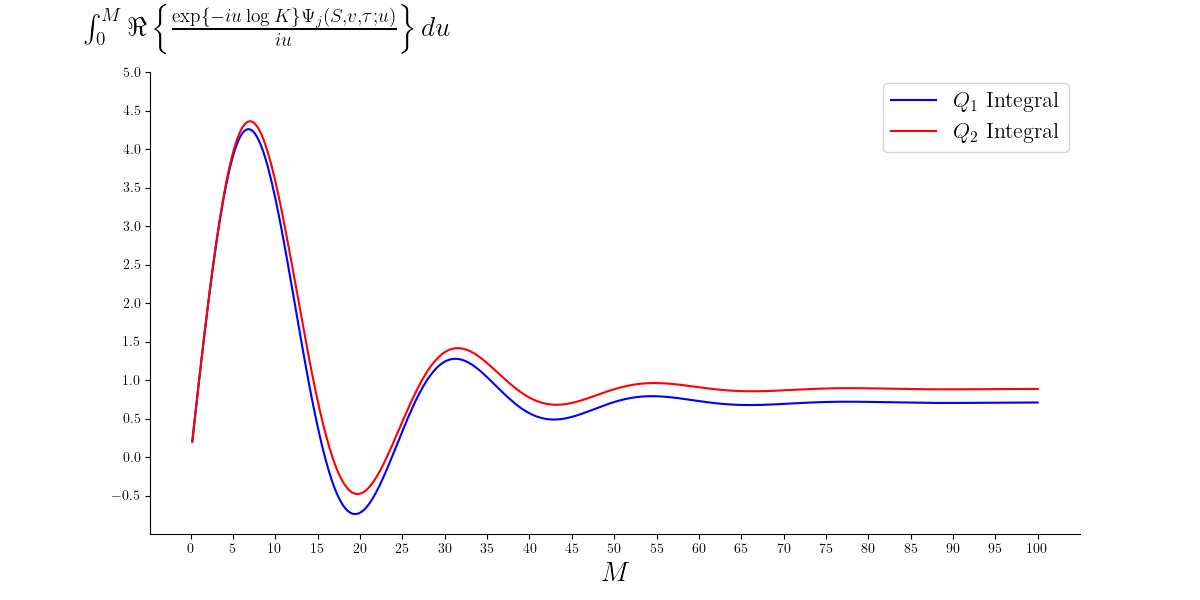
\includegraphics[width=\textwidth]{Qj-integrals.png}
    \caption{Fourier integral convergence properties illustrated by
    increasing the upper limit of the integral (shown along the $x$-axis and
    integral value on the $y$-axis). The fixed
    parameters used in the computation are set to: $\kappa = 2$, $\theta = 0.02$,
    $\rho = -0.5$, $\sigma = 0.3$, $\tau = 0.5$, $r = 0$, $v_0 = 0.01$, $S =
    100$, and $K = 80$.
    }
    \label{fig:qj-integrals}
\end{figure}

\newpage
\section{Option Pricing in the Heston Model Using Simulation}
Consider an arbitrary set of discrete times $\mathscr{T} = \{t_i\}_{i=1}^N$. We
need to generate random paths for the pair $(S_t, v_t)$ for all $t \in
\mathscr{T}$. This is important, for example, when pricing path-dependent
securities where the payout depends on observations of $S_t$ at specific dates.
To develop this approach, we first address the question of how to generate a
random sample of $(S_{t+\Delta}, v_{t+\Delta})$ given $(S_t, v_t)$ for any increment
$\Delta$. Repeatedly applying this one-period scheme (where $\Delta$ may vary at each
time in $\mathscr{T}$) will yield a complete path $(S_t, v_t)_{t \in
\mathscr{T}}$. Below, we outline several techniques for updating $S$ and $v$
from time $t$ to $t + \Delta$. But firstly, we introduce discretization
schemes of continuous time processes, then specific schemes and lastly Monte
Carlo methods. The implementations of the schemes in \texttt{Python} - the algorithms -
is seen in \autoref{sec:appendixscheme}.

\subsection{Discretization Schemes}
Assume that the model is defined on some filtered probability space
$(\Omega,\mathcal{F},\mathbb{F},\PP)$ and that the stock price $S_t$ is driven by the stochastic differential equation (SDE)
\begin{align}
dS_t = \underbrace{ \mu(S_t, t)}_{\text{drift}} dt + \underbrace{\sigma(S_t, t)}_{\text{diffusion}}dW_t^\PP,
\end{align}
where $W_t^\PP$ is a Wiener process. We simulate $S_t$ over the time interval $[0, T]$, which we assume is discretized as $0 = t_0 < t_1 < \dots < t_m = T$, with the time increments equally spaced with width $\Delta$. Equally-spaced time increments are primarily used for notational convenience, allowing us to write $t_{i} - t_{i-1}$ simply as $\Delta$.

Integrating (2.1) from $t$ to $t + \Delta$ yields:
\begin{align}
S_{t+\Delta} = S_t + \int_t^{t+\Delta} \mu(S_u, u)  du + \int_t^{t+\Delta} \sigma(S_u, u)  dW_u^\PP.
\end{align}
Equation (2.2) is the starting point for any discretization scheme. At time $t$,
the value of $S_t$ is known, and we aim to obtain the next value $S_{t+\Delta}$,
that is, the incremented value of $S_t$ to $S_{t+\Delta}$. This is the bread and
butter of both the simple discretization schemes: Euler and Milstein.

For the latter two schemes (or four if we count the \textit{Martingale corrected} versions of
the schemes) Truncated Gaussian (TG) and Quadratic-Exponential (QE) we need some
intermediate results of the variance process involving its conditional
distribution and moments. \cite{andersen2007efficient} Assumes that $\mu=0=r$ when
deriving his results, however, fear not: Assume that the forward price process
for the stock at expiry-$T$ is $F_t^T=S_te^{r(T-t)}$. Assume now that we apply
some discretization scheme to $F_t^T$ with increments $\Delta$ and note that
\begin{align*}
    S_{t+\Delta} &= F_{t+\Delta}^T e^{-r(T-(t+\Delta))}\\
    &=F_t^T \exp(\ \Box \ ) e^{-r(T-(t+\Delta))}\\
    &=S_t e^{r(T-t)}\exp(\ \Box \ ) e^{-r(T-(t+\Delta))}\\
    &=S_t \exp(r\Delta + \ \Box \ ),
\end{align*} 
where $\Box$ is exactly the terms in the discretization scheme where we started with $\mu=0=r$.

\newpage
Furthermore, we need the following proposition (found in \cite{cox1985theory}):
\begin{proposition}
Let $F_{\chi_{d}^{2}}$ be the cumulative distribution function of the non-central chi-squared distribution with non-centrality parameter $\lambda$ and $d$ degrees of freedom, i.e.
$$
F_{\chi_d^{2}}(x ; d, \lambda)=\sum_{i=0}^{\infty} e^{-\frac{\lambda}{2}} \frac{\left(\frac{\lambda}{2}\right)^{i}}{i!} \frac{\int_{0}^{x} t^{\frac{d}{2}+i-1} e^{-\frac{t}{2}} d t}{2^{\frac{d}{2}+i} \Gamma\left(i+\frac{d}{2}\right)}
$$
where $\Gamma$ is the gamma function. Let $t<T$. Conditional on $v_t$, $v_T$ is distributed as $\frac{\sigma^{2}\left(1-e^{-\kappa(T-t)}\right)}{4 \kappa}$ times a non-central chi-squared distributed random variable with $\frac{4 \kappa \theta}{\sigma^{2}}$ degrees of freedom and non-centrality parameter $\frac{4 \kappa e^{-\kappa(T-t)}}{\sigma^{2}\left(1-e^{-\kappa(T-t)}\right)} v_{t}$, i.e.
$$
\PP\left(v_T \leq x \mid v_t\right)=F_{\chi_d^{2}}\left(\frac{4 \kappa}{\sigma^{2} e^{-\kappa(T-t)}} x ; \frac{4 \kappa \theta}{\sigma^{2}}, \frac{4 \kappa e^{-\kappa(T-t)}}{\sigma^{2}\left(1-e^{-\kappa(T-t)}\right)} v_t\right)
$$
\end{proposition}

We prove a convenient corollary that follows simply from Proposition 2.1 as we now
know the distribution of $v_T$ given $v_t$:
\begin{corollary}
Let $T > t$. Conditional on $v_t$, $v_T$ has the following first two moments:
\begin{align*}
\EE(v_T \mid v_t) &= \theta + (v_t - \theta) e^{-\kappa(T-t)} \\
\operatorname{Var}(v_T \mid v_t) &= \frac{v_t \varepsilon^{2} e^{-\kappa(T-t)}}{\kappa}\left(1 - e^{-\kappa(T-t)}\right) + \frac{\theta \varepsilon^{2}}{2 \kappa}\left(1 - e^{-\kappa(T-t)}\right)^{2}
\end{align*}
\end{corollary}

\begin{proof}
Let $Y$ be a non-central $\chi_d^2(\lambda)$ distributed random variable with $d$ degrees
of freedom and non-centrality parameter $\lambda$. then
\begin{align*}
    \EE[Y]=d+\lambda, \quad \text{ and } \quad \operatorname{Var}=2(d+2\lambda)
\end{align*}
The conditional mean and
variance is then simply by Proposition 2.1 given as
$$
\begin{aligned}
\mathbb{E}\left[v_T \mid v_t\right] & =\frac{\sigma^{2}\left(1-e^{-\kappa(T-t)}\right)}{4 \kappa}\left(\frac{4 \kappa \theta}{\sigma^{2}}+\frac{4 \kappa e^{-\kappa(T-t)}}{\sigma^{2}\left(1-e^{-\kappa(T-t)}\right)} v_t\right) \\
& =\theta\left(1-e^{-\kappa(T-t)}\right)+v_t e^{-\kappa(T-t)},
\end{aligned}
$$
and
$$
\begin{aligned}
\operatorname{Var}\left(v_T \mid v_t\right) & =\frac{\sigma^{4}\left(1-e^{-\kappa(T-t)}\right)^{2}}{8 \kappa^{2}}\left(\frac{4 \kappa \theta}{\sigma^{2}}+\frac{8 \kappa e^{-\kappa(T-t)}}{\sigma^{2}\left(1-e^{-\kappa(T-t)}\right)} v_t\right) \\
& =\frac{\theta \sigma^{2}\left(1-e^{-\kappa(T-t)}\right)^{2}}{2 \kappa}+\frac{v_t\sigma^{2} e^{-\kappa(T-t)}}{\kappa}\left(1-e^{-\kappa(T-t)}\right).
\end{aligned}
$$
\end{proof}

Lastly, we have from \cite{johnson1995continuous}:

\begin{proposition} 
The non-central
chi-square distribution approaches a Gaussian distribution as the non-centrality
parameter approaches $\infty$.
\end{proposition}
From Proposition 2.1, we know that $v_{t+\Delta}$
is proportional to a non-central chi-square distribution with non-centrality
parameter $v_t\cdot \frac{4 \kappa
e^{-\kappa((t+\Delta)-t)}}{\sigma^{2}\left(1-e^{-\kappa((t+\Delta)-t)}\right)}
$, where the fraction is independent of $v_t$. This means,
for sufficiently large $v_t$, a good proxy for $v_{t+\Delta}$ would be a
Gaussian variable with the first two moments fitted to match those given in
Corollary 2.1 by Proposition 2.2.

Next we consider the contrary, namely small $v_t$. The non-centrality parameter
approaches zero, and the distribution of $v_{t+\Delta}$ becomes proportional to
that of an ordinary (central) chi-square distribution with $4 \kappa \theta /
\sigma^{2}$ degrees of freedom \cite{johnson1995continuous}. In other words

\begin{proposition}
    Let $\chi_d'^2(\lambda)$ denote a chi-squared random variable with $d$ degrees of
    freedom and centrality parameter $\lambda$. For $d>1$ the following
    representation is valid:
    \begin{align*}
        \chi_d'^2(\lambda)= \chi_1^2(\lambda)+\chi_{d-1}'^2(\lambda)
    \end{align*}
\end{proposition}
We recall that the density of a central chi-square distribution with $\nu$ degrees of freedom is
\begin{equation*}
f_{\chi^{2}}(x ; \nu)=\frac{1}{2^{\nu / 2} \Gamma(\nu / 2)} e^{-x / 2} x^{\nu / 2-1}.
\end{equation*}
For many cases of practical relevance, $4 \kappa \theta / \sigma^{2} \ll
2$, so the presence of the term $x^{\nu / 2-1}$ in the above equation implies that, for small
$v_t$, the density of $v_{t+\Delta}$ will be very large around 0. It should be clear that approximation of $v_{t+\Delta}$
with a Gaussian variable is typically not accurate when $v_t$ is close to zero. Note that all the results described above can be generalized to $0<s<t\leq T$.
\subsubsection{Euler Scheme}
The Monte Carlo Euler discretization scheme approximates the integrals using the
left-point rule, implying that the deterministic integral of (3.2) is
approximated as the product of the
integrand at time $t$, and the integration range $\Delta$:
\begin{align*}
    \int_t^{t+\Delta}\mu (S_t,u)du&\approx\mu(S_t,t)\int_t^{t+\Delta}du\\
    &=\mu(S_t,t)\Delta
\end{align*}
The left-point rule is a natural candidate as at time $t$ the value of
$\mu(S_t,t)$ is known (this is not the case for the right-point rule).

The stochastic integral is approximated in the exact same matter, i.e:
\begin{align*}
    \int_t^{t+\Delta}\sigma(S_u,u)dW_u^\PP&\approx \sigma(S_u,u) \int_t^{t+\Delta}\sigma(S_u,u)dW_u^\PP\\
    &=\sigma(S_u,u)(W_{t+\Delta}^\PP-W_t^\PP)\\
    &=\sigma(S_u,u)\sqrt{\Delta}Z^\PP,
\end{align*}
because $W_{t+\Delta}^\PP-W_t^\PP$ and $\sqrt{\Delta}Z^\PP$ are identically distributed,
where we define as $Z^\PP$ a standard normal random variable.

Assembling the results yields the general form of the Monte Carlo Euler
discretization scheme of (2.2):
\begin{align*}
    S_{t+\Delta} = S_t + \mu(S_t, t)  \Delta + \sigma(S_t, t) \sqrt{\Delta} Z^\PP
\end{align*}


We now proceed to apply Euler discretization to the Heston model given in
equation (1.1). The stochastic differential equation of the variance is in integral form
given by
\begin{align*}
    v_{t+\Delta}=v_t+\int_t^{t+\Delta}\kappa(\theta-v_u)du+\int_t^{t+\Delta}\sigma\sqrt{v_u}dW_{2,u}^\PP.
\end{align*}
The Monte Carlo Euler discretization approximates the integrals by linearity using the
left-point rule as
\begin{align*}
    \int_t^{t+\Delta}\kappa(\theta-v_u)du\approx \kappa(\theta-v_t)\Delta,
\end{align*}
and
\begin{align*}
    \int_t^{t+\Delta}\sigma\sqrt{v_u}dW_{2,u}^\PP &\approx \sigma \sqrt{v_t}(W_{2,t+\Delta}^\PP-W_{2,t}^\PP)\\
    &=\sigma \sqrt{v_t \Delta}Z_v^\PP,
\end{align*}
as we do not know $v_{t+\Delta}$ at time $t$ and where $Z_v^\PP$ is a standard normal
random variable. These results yield the process for the variance
\begin{align*}
    v_{t+\Delta}=v_t+\kappa(\theta-v_t)\Delta +\sigma\sqrt{v_t \Delta}Z_v^\PP
\end{align*}


The stochastic differential equation of the stock price is in integral form
given by
\begin{align*}
    S_{t+\Delta}=S_t+\mu\int_t^{t+\Delta}S_u du+\int_t^{t+\Delta}\sqrt{v_u}S_udW_{1,u}^\PP.
\end{align*}
The Monte Carlo Euler discretization approximates the integrals by linearity
using the left-point rule as
\begin{align*}
    \int_t^{t+\Delta}S_u du\approx S_t \Delta,
\end{align*}
and
\begin{align*}
    \int_t^{t+\Delta} \sqrt{v_u}S_udW_{1,u}^\PP&\approx \sqrt{v_t}S_t(W_{1,t+\Delta}^\PP-W_{1,t}^\PP)\\
    &=\sqrt{v_t\Delta}S_tZ_s^\PP,
\end{align*}
where $Z_s^\PP$ is a standard normal random variable with correlation $\rho$ with
the prievously defined random variable $Z_v^\PP$. These results yield the process
for the stock price
\begin{align*}
    S_{t+\Delta}=S_t+\mu S_t \Delta +\sqrt{v_t \Delta }S_tZ_s^\PP.
\end{align*} 

We simulate $S_t$ over the time interval $[0, T]$ (to
and including expiry),
which we assume to be discretized as $0 = t_1 < t_2 < \ldots < t_m = T$, where
the time increments are equally spaced with width $\Delta$. For $n\in\NN$ we use
the Euler discretization on an equidistan time grid $\lc t_i=\frac{iT}{n}\mid
i=0,\ldots,n\rc$, where $n$ is the number of time points after $t=0$. We start with the initial
values $S_0$ for the stock price and $v_0$ for the variance. To generate
$Z_v^\PP$ and $Z_s^\PP$ with correlation $\rho$, we first generate two
independent standard normal variables $Z_1^\PP$ and $Z_2^\PP$ and set $Z_v^\PP
= Z_1^\PP$ and $Z_s^\PP = \rho Z_1^\PP + \sqrt{1 - \rho^2} Z_2^\PP$ by Cholesky decomposition.
For an arbitrary but fixed $\lambda$ (i.e no estimation of $\lambda$ needed) we
use the adjusments (as suggested in \cite{heston1993closed}):
\begin{align*}
    \tilde{\kappa}=\kappa+\lambda \quad \text{ and } \quad \tilde{\theta}=\frac{\kappa\theta}{\kappa + \lambda},
\end{align*}
and thus by the fact that the drift under the risk neutral measure is equal to
the risk-free rate
\begin{align*}
    S_{t+\Delta}&=S_t+rS_t\Delta+\sqrt{v_t \Delta}S_t Z_s^{\tilde{\QQ}},\\
    v_{t+\Delta} &= v_t +\tilde{\kappa}(\tilde{\theta} - v_t)\Delta + \sigma \sqrt{v_t \Delta}Z_v^{\tilde{\QQ}},
\end{align*}
yielding that the price under the equivalent martingale measure
$\tilde{\QQ}(\lambda)$ is unique, i.e choosing a different arbitrary
$\lambda^\star\neq \lambda$ would yield another equivalent martingale measure
$\tilde{\QQ}(\lambda^\star)$ among the infinite number of measures.

Lastly, we note that there might occure negative $v$-values at some of the time
points due to discretization errors. When
this occurs we use a full truncation scheme, namely, $\max\lc 0,v_t\rc$ but
firstly count it towards
our zero-variance-count for later reporting.
\newpage
\subsubsection{Milstein Scheme}
We assume the coefficients $\mu(S_t),\sigma(S_t)$ only depend on $S$ and not
direcctly on $t$ and is described the SDE
\begin{align}
    dS_t &= \mu(S_t)\Delta+\sigma(S_t)dW_t^\PP
\end{align}
or in integral notation with the shorthand $\mu_t=\mu(S_t),\sigma_t=\sigma(S_t)$
\begin{align*}
    S_{t+\Delta}=S_t+\int_t^{t+\Delta}\mu_s ds+\int_t^{t+\Delta}\sigma_s dW_s^\PP.
\end{align*}
By Itō's lemma, we find the expansion of $\mu_t,\sigma_t$
\begin{align*}
    d\mu_t &= \left ( \mu_t'\mu_t+\frac{1}{2}\mu_t''\sigma_t^2 \right )\Delta+(\mu_t'\sigma_t)dW_t^\PP\\
    d\sigma_t &=\left ( \sigma_t'\mu_t+\frac{1}{2}\sigma_t''\sigma_t^2 \right )\Delta+(\sigma_t'\sigma_t)dW_t^\PP
\end{align*}
At time $s$ where $t<s<t+\Delta$ the integral form of the coefficients is
\begin{align*}
    \mu_s &=\mu_t+\int_t^s \left ( \mu_u'\mu_u+\frac{1}{2}\mu_u''\sigma_u^2\right )du+\int_t^s (\mu_u'\sigma_u)dW_u^\PP\\
    \sigma_s &= \sigma_t + \int_t^{s} \left ( \sigma_u'\mu_u+\frac{1}{2}\sigma_u''\sigma_u^2 \right )du+ \int_t^s (\sigma_u'\sigma_u)dW_u^\PP
\end{align*}
Substituting the integral form expanded expressions for the coefficients into
(2.3) yields
\begin{align*}
    S_{t+\Delta}&=S_t+\int_t^{t+\Delta}\left ( \mu_t+\int_t^s \left ( \mu_u'\mu_u+\frac{1}{2}\mu_u''\sigma_u^2\right )du+\int_t^s (\mu_u'\sigma_u)dW_u^\PP\right )ds\\
    &\quad + \int_t^{t+\Delta}\left (  \sigma_t + \int_t^{s} \left ( \sigma_u'\mu_u+\frac{1}{2}\sigma_u''\sigma_u^2 \right )du+ \int_t^s (\sigma_u'\sigma_u)dW_u^\PP \right )dW_s^\PP.
\end{align*}
We ignore terms higher than order one, meaning, we ignore $dsdu=\mathcal{O}\left
((\Delta)^2 \right )$ and $dsdW_u^\PP=\mathcal{O} \left ( (\Delta)^{3/2} \right )$ and
thus
\begin{align}
    S_{t+\Delta}&=S_t+\mu_t \int_t^{t+\Delta}+\sigma_t \int_t^{t+\Delta}dW_s^\PP+\underbrace{\int_t^{t+\Delta}\int_t^s (\sigma_u'\sigma_u)dW_u^\PP dW_s^\PP}_{(*)}.
\end{align}
Applying Euler discretization from subsection (2.1.2) to $(*)$ in equation (2.4)
yields
\begin{align*}
    \int_t^{t+\Delta}\int_t^s (\sigma_u'\sigma_u)dW_u^\PP dW_s^\PP &\approx \sigma_t'\sigma_t \int_t^{t+\Delta}\int_t^s dW_u^\PP dW_s^\PP\\
    &=\sigma_t'\sigma_t \int_t^{t+\Delta}(W_s^\PP-W_t^\PP) dW_s^\PP\\
    &=\sigma_t'\sigma_t \left (\int_t^{t+\Delta} W_s^\PP d W_s^\PP-W_t^\PP W_{t+\Delta}^\PP+ \left(W_t^\PP\right)^2 \right )
\end{align*}
Define $dY_t=W_t^\PP dW_t^\PP$. Using Itō's lemma we see that
$Y_t=\frac{1}{2}\left ( W_t^\PP \right)^2-\frac{1}{2}t$ as $\frac{\partial Y}{\partial
t}=-\frac{1}{2}$, $\frac{\partial Y_t}{\partial
W_t ^\PP}=W_t ^\PP$ and $\frac{\partial ^2 Y_t}{\partial \left ( W_t ^\PP\right )^2}=1$, such that
\begin{align*}
    dY_t=\left( -\frac{1}{2}+0+\frac{1}{2}\cdot 1 \cdot 1\right)\Delta+(W_t^\PP \cdot 1)dW_t^\PP=W_t^\PP dW_t ^\PP
\end{align*}
This means we can further rewrite the term $(*)$ in equation (2.4) as
\begin{align*}
    \int_t^{t+\Delta}\int_s^t \sigma_u'\sigma_u dW_u^\PP dW_s^\PP&\approx \frac{1}{2}\sigma_u'\sigma_u \left [ (\underbrace{W_{t+\Delta}-W_t}_{(**)})^2-\Delta \right ],
\end{align*}
where $(**)$ is equal in distribution to $\sqrt{\Delta}Z$ where $Z$ is distributed
as standard normal. Combinding our rewritings of $(*)$ in equation (2.4) we
achieve the general form of Milstein discretization scheme
\begin{align}
    S_{t+\Delta}=S_t+\mu_t \Delta +\sigma-t \sqrt{\Delta}Z+\frac{1}{2}\sigma_t'\sigma_t \Delta \left( Z^2-1\right).
\end{align}

We now proceed to apply Milstein discretization to the Heston model given in
equation (1.1). Given a value $v_t$ we proceed to $v_{t+\Delta}$ by
\begin{align*}
    v_{t+\Delta}=v_t+\tilde{\kappa}(\tilde{\theta}-v_t)\Delta+\sigma \sqrt{v_t \Delta}Z_v^{\tilde{\QQ}}+\frac{1}{4}\sigma^2\Delta\left( \left ( Z_v^2 \right)^{\tilde{\QQ}}-1\right),
\end{align*}
and given a value $S_t$ we proceed to $S_{t+\Delta}$ by 
\begin{align*}
    S_{t+\Delta}=S_t+r S_t \Delta + \sqrt{v_t \Delta} S_tZ_s^{\tilde{\QQ}}+\frac{1}{4}S_t^2\Delta \left ( (Z_s^{\tilde{\QQ}})^2-1\right ).
\end{align*}
We generate the random variables, under $\tilde{\QQ}(\lambda)$, with correlation
$\rho$ exactly as described in subsection 2.1.1 and use the altered
$\tilde{\kappa},\tilde{\theta}$.
\subsubsection{Truncated Gaussian Scheme}

\subsubsection{Truncated Gaussian Scheme: Martingale Corrected}
\subsubsection{Quadratic-Exponential Scheme}
\subsubsection{Quadratic-Exponential Scheme: Martingale Corrected}
\newpage
\subsubsection{Monte Carlo Simulation for Pricing}
Our goal is to find a solution to the Heston process, by using the schemes
presented above together with Monte Carlo simulation. The solution of the SDE
will (hopefully) converge towards the real value. By simulating the process a
large number of times, the value will eventually converge towards the real
value, $C(0)$. The basic idea of Monte Carlo is to approximate an integral by
taking the average of some sequence of simulated paths.

For example, say we wanted to evaluate the following integral/expectation:
\begin{align*}
I = \mathbb{E}[\Phi(X)] = \int \Phi(X) f(X)  dx,
\end{align*}

where $X \in \mathbb{R}^d$, $\Phi : \mathbb{R}^d \to \mathbb{R}$, and $f$ is the probability density function of $X$. $I = \mathbb{E}[\Phi(X)]$ can then be approximated in the following way:

\begin{itemize}
    \item[1. ] Draw $N$ values $X_1, \ldots, X_N$ i.i.d. from $f$.
    \item[2. ] The integral can then be evaluated as
 \begin{align*}
        I \approx \frac{1}{N} \sum_{i=1}^{N} \Phi(X_i).
        \end{align*}
\end{itemize}

So, to compute an estimate of the European call option price, $\hat{C}(0)=\EE_0^\QQ
\Big( (\hat{S}_T-K)^+ \Big)$, we use Monte Carlo methods.
Specifically, for some given discretization scheme of $S_t$ (denote this discretization by $\hat{S_t}$), we draw $N$ independent
samples of $\hat{S}_T^{(1)},\hat{S}_T^{(2)}, \ldots, \hat{S}_T^{(N)}$
using an equidistant time-grid $\left \{ t_i = \frac{iT}{n}, \: i=0,\ldots,n
\right \}$ with fixed step $\Delta$ where $n\in \NN$, then $\hat{C}(0)$ is estimated
in a Monte Carlo fashion as
\begin{align*}
    \hat{C}(0)\approx \frac{1}{N}\sum_{i=1}^{N} \Big(\hat{S}_T^{(i)}-K \Big)^+.
\end{align*}
The right-hand side of this equation is a random variable with mean $\hat{C}(0)$
and a standard deviation ("Monte Carlo error") of order $\mathcal{O}(N^{-1/2})$
by the Central Limit Theorem.
Using a sufficiently high number $ N $ of samples, we can keep the standard
deviation low and obtain a high-accuracy estimate for $\hat{C}(0)$ by the Law of
Large Numbers.

\section{Numerical Tests}
\section{Discussion}
\section{Conclusion}
\appendix
\section{Appendix: Code}\label{chap:code}
\href{https://github.com/YoussefRaad-mathecon/Handin-3}{GitHub repository holding implementation of every simulation scheme and exact call option calculations.}

\newpage
\section{Appendix: Scheme Algorithms}\label{sec:appendixscheme}
We outline the algorithm implementation in \texttt{Python}. This does not include in depth methodology to gain efficieny and supplementary functions such as pricing and zero variance count. We omit notation of which measure we are under as that is described excessively in the theoretical parts of the paper.

\begin{algorithm}
\caption{Euler scheme (\texttt{generateHestonPathEulerDisc})}
\begin{algorithmic}
\State \textbf{Inputs:} $S_0, v_0, r, \kappa, \theta, \sigma, \rho, T, n$
\State Set $S_0 = S_0$
\State Set $v_0 = v_0$
\State Generate $\mathbf{Z}_1\sim \mathcal{N}(\mathbf{0}, \mathbf{I})$
\State Generate $\mathbf{Z}_2 \sim \mathcal{N}(\mathbf{0}, \mathbf{I})$
\State Set $\mathbf{Z}_v = \mathbf{Z}_1$
\State Set $\mathbf{Z}_s = \rho \mathbf{Z}_1 + \sqrt{1 - \rho^2} \mathbf{Z}_2$
\For{$i = 1$ to $n$}
    \State $v_{t+i}=v_t^++\kappa(\theta-v_t^+)\Delta+\sigma \sqrt{v_t^+ \Delta}Z_v^{(i)}$
    \State $S_{t+i}=S_t+rS_t\Delta+\sqrt{v_t^+ \Delta}S_tZ_s^{(i)}$
\EndFor
\State \Return $S_n$
\end{algorithmic}
\end{algorithm}

\begin{algorithm}
\caption{Milstein scheme (\texttt{generateHestonPathMilsteinDisc})}
\begin{algorithmic}
\State \textbf{Inputs:} $S_0, v_0, r, \kappa, \theta, \sigma, \rho, T, n$
\State Set $S_0 = S_0$
\State Set $v_0 = v_0$
\State Generate $\mathbf{Z}_1\sim \mathcal{N}(\mathbf{0}, \mathbf{I})$
\State Generate $\mathbf{Z}_2 \sim \mathcal{N}(\mathbf{0}, \mathbf{I})$
\State Set $\mathbf{Z}_v = \mathbf{Z}_1$
\State Set $\mathbf{Z}_s = \rho \mathbf{Z}_1 + \sqrt{1 - \rho^2} \mathbf{Z}_2$
\For{$i = 1$ to $n$}
    \State $v_{t+i}=v_t^++\kappa(\theta-v_t)\Delta+\sigma \sqrt{v_t^+ \Delta}Z_v^{(i)}+\frac{1}{4}\sigma^2 \Delta \left( \left( Z_s^{(i)}\right)^2-1\right)$
    \State $S_{t+i}=S_t+rS_t\Delta+\sqrt{v_t^+ \Delta}S_tZ_s^{(i)}+\frac{1}{4}S_t^2\Delta \left (\left( Z_s^{(i)}\right)^2-1\right)$
\EndFor
\State \Return $S_n$
\end{algorithmic}
\end{algorithm}

\newpage
\begin{algorithm}
\caption{Truncated Gaussian scheme (\texttt{generateHestonPathTGDisc})}
\begin{algorithmic}
\State \textbf{Inputs:} $S_0, v_0, r, \kappa, \theta, \sigma, \rho, T, n,\gamma_1,\gamma_2,\alpha$
\State Set $S_0 = S_0$
\State Set $v_0 = v_0$
\State Set $\gamma_1=\gamma_1\in (0,1)$
\State Set $\gamma_2=1-\gamma_1 \in (0,1)$
\State Set $\alpha=\alpha$ around 4 or 5
\State Compute $K_0 =  \frac{-\rho \kappa \theta}{\sigma} \Delta$
\State Compute $K_1 = \gamma_1 \Delta \left (\frac{\kappa \rho }{\sigma}-\frac{1}{2} \right)-\frac{\rho}{\sigma}$
\State Compute $K_2=\gamma_2\Delta \left ( \frac{\kappa \rho }{\sigma}-\frac{1}{2}\right )+\frac{\rho}{\sigma}$
\State Compute $K_3=\gamma_1\Delta (1-\rho^2)$
\State Compute $K_4=\gamma_2\Delta (1-\rho^2)$
\State Generate $\mathbf{Z}_s \sim \mathcal{N}(\mathbf{0}, \mathbf{I})$
\State Generate $\mathbf{U}_v \sim \mathcal{U}(0, 1)^n$
\State Set $\mathbf{Z}_v = \Phi^{-1}(\mathbf{U}_v)$ where $\Phi^{-1}$ is the inverse CDF of the standard normal distribution
\For{$i = 1$ to $n$}
\State Compute $m = \theta + (v_t - \theta)e^{-\kappa \Delta} $
\State Compute $s^2 = \frac{v_t\sigma^2 e^{-\kappa \Delta}}{\kappa}\left (1-e^{-\kappa \Delta}\right)+\frac{\theta \sigma ^2}{2\kappa}\left(1-e^{-\kappa \Delta}\right)$
\State Set $\psi = \frac{s^2}{m^2}$

\If{$\psi^{-1/2}>\alpha$}
\State Set $\mu=m$
\State Set $\sigma=s$
\vspace{0.1cm}
\State $v_{t+i}=\left(\mu+\sigma Z_v^{(i)} \right )$
\Else
\State Compute $f_\mu(\psi)=\frac{r(\psi)}{\phi(r(\psi))+r(\psi)\Phi(r(\psi))}$
\State Compute $f_\sigma(\psi)=\frac{\psi^{-1/2}}{\phi(r(\psi))+r(\psi)\Phi(r(\psi))}$
\State Set $\mu=f_\mu(\psi)\cdot m$
\State Set $\sigma=f_\sigma(\psi)\cdot s$
\vspace{0.1cm}
\State $v_{t+i}=\left(\mu+\sigma Z_v^{(i)} \right )$
\EndIf
\State $S_{t+i}=S_t \exp\left(r \cdot \Delta + K_0 + K_1 \cdot v_t  \right) \exp\left(K_2 \cdot v_{t+\Delta}+\sqrt{K_3 \cdot v_t + K_4 \cdot v_{t+\Delta}} \cdot Z_s^{(i)}\right)$
\EndFor
\State \Return $S_n$
\end{algorithmic}
\end{algorithm}

\begin{algorithm}
\caption{Quadratic-Exponential scheme (\texttt{generateHestonPathQEDisc})}
\begin{algorithmic}
\State \textbf{Inputs:} $S_0, v_0, r, \kappa, \theta, \sigma, \rho, T, n,\gamma_1,\gamma_2,\alpha$
\State Set $S_0 = S_0$
\State Set $v_0 = v_0$
\State Set $\gamma_1=\gamma_1\in (0,1)$
\State Set $\gamma_2=1-\gamma_1 \in (0,1)$
\State Set $\psi_C=\psi_C\in [1,2]$ 
\State Compute $K_0 =  \frac{-\rho \kappa \theta}{\sigma} \Delta$
\State Compute $K_1 = \gamma_1 \Delta \left (\frac{\kappa \rho }{\sigma}-\frac{1}{2} \right)-\frac{\rho}{\sigma}$
\State Compute $K_2=\gamma_2\Delta \left ( \frac{\kappa \rho }{\sigma}-\frac{1}{2}\right )+\frac{\rho}{\sigma}$
\State Compute $K_3=\gamma_1\Delta (1-\rho^2)$
\State Compute $K_4=\gamma_2\Delta (1-\rho^2)$
\State Generate $\mathbf{Z}_s \sim \mathcal{N}(\mathbf{0}, \mathbf{I})$
\State Generate $\mathbf{U}_v \sim \mathcal{U}(0, 1)^n$
\State Set $\mathbf{Z}_v = \Phi^{-1}(\mathbf{U}_v)$ where $\Phi^{-1}$ is the inverse CDF of the standard normal distribution
\For{$i = 1$ to $n$}
\State Compute $m = \theta + (v_t - \theta)e^{-\kappa \Delta} $
\State Compute $s^2 = \frac{v_t\sigma^2 e^{-\kappa \Delta}}{\kappa}\left (1-e^{-\kappa \Delta}\right)+\frac{\theta \sigma ^2}{2\kappa}\left(1-e^{-\kappa \Delta}\right)$
\State Set $\psi = \frac{s^2}{m^2}$

\If{$\psi \leq \psi_C$}
\State Set $b^2=2\psi^{-1}-1+\sqrt{2\psi^{-1}}\sqrt{2\psi^{-1}-1}\geq 0$
\State Set $a=\frac{m}{1+b^2}$
\vspace{0.1cm}
\State $v_{t+i}=a\left(b+ Z_v^{(i)} \right )^2$
\Else
\State Compute $p=\frac{\psi-1}{\psi+1}\in [0,1)$
\State Compute $\beta=\frac{1-p}{m}>0$
\If{$0\leq U_v^{(i)}\leq p$}
\State $v_{t+i}=0$
\Else
\State $v_{t+i}=\beta^{-1}\ln\left ( \frac{1-p}{1-U_v^{(i)}}\right )$
\EndIf
\EndIf
\State $S_{t+i}=S_t \exp\left(r \cdot \Delta + K_0 + K_1 \cdot v_t  \right) \exp\left(K_2 \cdot v_{t+\Delta}+\sqrt{K_3 \cdot v_t + K_4 \cdot v_{t+\Delta}} \cdot Z_s^{(i)}\right)$
\EndFor
\State \Return $S_n$
\end{algorithmic}
\end{algorithm}

\newpage
\bibliographystyle{abbrvnat}

\bibliography{mybib.bib}
\end{document}